\section{字符串简介}

\begin{frame}[fragile,allowframebreaks] \ft{\secname}
\lstinputlisting[language=C,frame=single,numbers=left]{
Code/talkback.c
}
\end{frame}


\begin{frame}[fragile] \ft{\secname}
\begin{lstlisting}
Hi! What's your name?
Xiaoping
Xiaoping, what's your weight in pounds?
139
Well, Xiaoping, your volume is 2.23 cubic feet.
Also, your first name has 8 letters, 
and we have 40 bytes to store it in.
\end{lstlisting}
\end{frame}

\begin{frame}[fragile] \ft{\secname}
\begin{dingyi}
字符串(character string)就是一个或多个字符的序列。例如:
\begin{lstlisting}
"Once more you open the door!"
\end{lstlisting}

\end{dingyi}
\vspace{0.1in}

\begin{zhu}
字符串用双引号括起来,但双引号不是字符串的一部分。
\end{zhu}
\end{frame}

\begin{frame} \ft{\secname}
\begin{itemize}
\item
C没有为字符串定义专门的数据类型,而是把它存储在char数组中。
\\[0.2in]
\item
字符串的字符存放在相邻的存储单元中,每个字符占用一个单元。
\\[0.2in]
\item
而数组由相邻存储单元组成,故把字符串存储在数组中是自然的。
\end{itemize}
\end{frame}



\begin{frame}\ft{\secname}
\begin{figure}
\centering
\begin{tikzpicture}
\def\x{0.37}
\foreach \i in {0,1,...,28}{
\draw[fill=gray!10] (\i*\x,0)rectangle(\i*\x+\x,\x);
\ifthenelse{\i=0} {\node at (\i*\x+0.5*\x,0) [above]{O};}{}
\ifthenelse{\i=1} {\node at (\i*\x+0.5*\x,0) [above]{n};}{}
\ifthenelse{\i=2} {\node at (\i*\x+0.5*\x,0) [above]{c};}{}
\ifthenelse{\i=3} {\node at (\i*\x+0.5*\x,0) [above]{e};}{}
\ifthenelse{\i=4} {
\node at (\i*\x+0.5*\x,0) [above]{ };
\draw[->,>=stealth,very thick](\i*\x+0.5*\x,-1.2*\x)--(\i*\x+0.5*\x,0);
\node at (\i*\x+0.5*\x,-2*\x){每个单元占1个字节};

}{}
\ifthenelse{\i=5} {\node at (\i*\x+0.5*\x,0) [above]{m};}{}
\ifthenelse{\i=6} {\node at (\i*\x+0.5*\x,0) [above]{o};}{}
\ifthenelse{\i=7} {\node at (\i*\x+0.5*\x,0) [above]{r};}{}
\ifthenelse{\i=8} {\node at (\i*\x+0.5*\x,0) [above]{e};}{}
\ifthenelse{\i=9} {\node at (\i*\x+0.5*\x,0) [above]{ };}{}
\ifthenelse{\i=10}{\node at (\i*\x+0.5*\x,0.4*\x) []{y};}{}
\ifthenelse{\i=11}{\node at (\i*\x+0.5*\x,0) [above]{o};}{}
\ifthenelse{\i=12}{\node at (\i*\x+0.5*\x,0) [above]{u};}{}
\ifthenelse{\i=13}{\node at (\i*\x+0.5*\x,0) [above]{ };}{}
\ifthenelse{\i=14}{\node at (\i*\x+0.5*\x,0) [above]{o};}{}
\ifthenelse{\i=15}{\node at (\i*\x+0.5*\x,0.4*\x) []{p};}{}
\ifthenelse{\i=16}{\node at (\i*\x+0.5*\x,0) [above]{e};}{}
\ifthenelse{\i=17}{\node at (\i*\x+0.5*\x,0) [above]{n};}{}
\ifthenelse{\i=18}{\node at (\i*\x+0.5*\x,0) [above]{ };}{}
\ifthenelse{\i=19}{\node at (\i*\x+0.5*\x,0) [above]{t};}{}
\ifthenelse{\i=20}{\node at (\i*\x+0.5*\x,0) [above]{h};}{}
\ifthenelse{\i=21}{\node at (\i*\x+0.5*\x,0) [above]{e};}{}
\ifthenelse{\i=22}{\node at (\i*\x+0.5*\x,0) [above]{ };}{}
\ifthenelse{\i=23}{\node at (\i*\x+0.5*\x,0) [above]{d};}{}
\ifthenelse{\i=24}{\node at (\i*\x+0.5*\x,0) [above]{o};}{}
\ifthenelse{\i=25}{\node at (\i*\x+0.5*\x,0) [above]{o};}{}
\ifthenelse{\i=26}{\node at (\i*\x+0.5*\x,0) [above]{r};}{}
\ifthenelse{\i=27}{\node at (\i*\x+0.5*\x,0) [above]{!};}{}

\ifthenelse{\i=28}{
\node at (\i*\x+0.5*\x,0) [above]{$\backslash$0};
\draw[->,>=stealth,very thick](\i*\x+0.5*\x,-1.2*\x)--(\i*\x+0.5*\x,0);
\node at (\i*\x+0.5*\x,-2*\x){空字符};
}{}

}
\end{tikzpicture}
\end{figure}
\end{frame}

\begin{frame}[fragile]\ft{\secname}
\begin{itemize}
\item 数组中的最后一个位置显示字符$\backslash$0,该字符是空字符(null character),C用它来标记字符串的结束。\\[0.15in]
\item 空字符不是数字0,它是非打印字符,其ASCII码的值为0。\\[0.15in]
\item 空字符的存在意味着数组的单元数至少比要存储的字符数多1。
\end{itemize}

\end{frame}


\begin{frame}\ft{\secname}
\begin{dingyi}
\textcolor{acolor1}{数组(array)}是同一类型的数据元素的有序序列。
\end{dingyi}
\end{frame}


\begin{frame}[fragile]\ft{\secname:如何创建数组?}
\begin{lstlisting}[backgroundcolor=\color{red!10}]
char name[40];
\end{lstlisting}
该声明语句创建一个有40个存储单元的数组,其中每个单元可存储一个char型值。
\pause \vspace{0.1in}

\begin{itemize}
\item 方括号说明name是一个数组\\[0.1in]
\item 方括号中的40指出数组中的元素个数\\[0.1in]
\item char标识每个元素的类型
\end{itemize}
\end{frame}


\begin{frame}[fragile]\ft{\secname:字符串的使用}
要使用字符串,必须创建一个数组,把字符串中的字符逐个放入数组中,最后还需在结尾添加一个空字符$\backslash$0。
\end{frame}

\begin{frame}[fragile]\ft{\secname:字符串的使用}
\lstinputlisting[language=c,frame=single,numbers=left]{
Code/praise1.c
}
\end{frame}

\begin{frame}[fragile]\ft{\secname:字符串的使用}

\begin{lstlisting}[backgroundcolor=\color{red!10}]
$ gcc praise1.c
$ ./a.out
What's your name?
Xiaoping Zhang
Hello, Xiaoping. What a super marvelous name!
\end{lstlisting}

\end{frame}

\begin{frame}[fragile]\ft{\secname:字符串的使用}
关于scanf()函数

\begin{itemize}
\item \tf 无须把空字符插入name数组中,scanf会在读取输入时完成此任务。\\[0.1in]
\item name前无须加\&,因为name本身就是地址。\\[0.1in]
\item 使用\%s的scanf语句会在遇到的第一个空格、制表符或换行符处停止读取,它只会把第一个单词而不是把整条语句作为字符串读入。\\[0.1in]
\item[] 因此,该程序只读取了Xiaoping。

\end{itemize}
\end{frame}

\begin{frame}[fragile]\ft{\secname:字符与字符串}
请注意"x"与'x'的差别\vspace{0.1in}

\begin{itemize}
\item 'x'为字符,而"x"为字符串\\[0.1in]
\item "x"由两个字符'x'和'$\backslash$0'组成

\end{itemize}
\end{frame}

\begin{frame}[fragile]\ft{\secname:strlen函数}
\begin{itemize}
\item 对sizeof运算符,以字节为单位给出数据大小;\\[0.1in]
\item 对strlen函数,以字符为单位给出字符串的长度,不包含空字符。

\end{itemize}

\end{frame}

\begin{frame}[fragile,allowframebreaks]\ft{\secname:strlen函数}
\lstinputlisting[language=c,frame=single,numbers=left]
    {
      Code/praise2.c
    }
\end{frame}


\begin{frame}[fragile]\ft{\secname:strlen函数}

\begin{lstlisting}[backgroundcolor=\color{red!10}]
$ gcc praise2.c
$ ./a.out
What's your name?
Xiaoping
Hello, Xiaoping. What a super marvelous name!
Your name of 8 letters occupied 40 memory cells.
The phrase of PRAISE has 28 letters and occpied 29 memory cells.
\end{lstlisting}
\end{frame}

\begin{frame}[fragile]\ft{\secname:strlen函数}
\begin{itemize}
\item \tf 头文件string.h包含许多与字符串相关的函数的原型,包括strlen函数。\\[0.1in]
\item C把函数库分成多个相关函数的序列,并为每个序列提供一个头文件。比如:\\[0.1in]
\item[(1)] printf和scanfs属于标准输入输出序列,使用stdio.h。\\[0.1in]
\item[(2)] strlen和其它一些与字符串相关的函数同属一个系列,使用string.h。
\end{itemize}
\end{frame}

\begin{frame}[fragile]\ft{\secname:printf函数处理长字符串}
\begin{itemize}
\item 一条printf语句占用两行,但只能在参数之间断行,不允许在字符串中间断行。\\[0.1in]
\item 使用两个printf语句输出一行,换行符只出现在第二条语句。
\end{itemize}
\end{frame}

\begin{frame}[fragile]\ft{\secname:sizeof运算符与strlen返回值}
设name = "Morgan",则
\begin{lstlisting}[backgroundcolor=\color{red!10}]
sizeof name : 40
strlen(name): 6
\end{lstlisting}

\begin{figure}
\centering
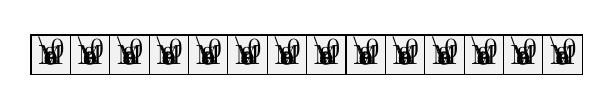
\begin{tikzpicture}
\def\x{0.5}
\foreach \i in {0,1,...,13}{
\draw[fill=gray!10] (\i*\x,0)rectangle(\i*\x+\x,\x);
\ifthenelse{\i=0} {\node at (\i*\x+0.5*\x,0) [above]{M};}{}
\ifthenelse{\i=1} {\node at (\i*\x+0.5*\x,0) [above]{o};}{}
\ifthenelse{\i=2} {\node at (\i*\x+0.5*\x,0) [above]{r};}{}
\ifthenelse{\i=3} {\node at (\i*\x+0.5*\x,0) [above]{g};}{}
\ifthenelse{\i=4} {\node at (\i*\x+0.5*\x,0) [above]{a};}{}
\ifthenelse{\i=5} {\node at (\i*\x+0.5*\x,0) [above]{n};}{}
\ifthenelse{\i=6} {\node at (\i*\x+0.5*\x,0) [above]{$\backslash$0};}{}
\ifthenelse{\i=7} {\node at (\i*\x+0.5*\x,0) [above]{};}{}
\ifthenelse{\i=8} {\node at (\i*\x+0.5*\x,0) [above]{};}{}
\ifthenelse{\i=9} {\node at (\i*\x+0.5*\x,0) [above]{};}{}
\ifthenelse{\i=10}{\node at (\i*\x+0.5*\x,0.4*\x) []{};}{}
\ifthenelse{\i=11}{\node at (\i*\x+0.5*\x,0) [above]{};}{}
\ifthenelse{\i=12}{\node at (\i*\x+0.5*\x,0) [above]{};}{}
\ifthenelse{\i=13}{\node at (\i*\x+0.5*\x,0) [above]{ };}{}
}
\end{tikzpicture}
\end{figure}
\end{frame}

\begin{frame}[fragile]\ft{\secname:sizeof运算符与strlen返回值}
\begin{lstlisting}[backgroundcolor=\color{red!10}]
sizeof PRAISE : 29
strlen(PRAISE): 28
\end{lstlisting}

sizeof运算符在处理字符串变量时,会将空字符也计算在内。
\end{frame}

\begin{frame}[fragile]\ft{\secname:sizeof运算符后的圆括号}
\begin{itemize}
\item 圆括号对于数据类型是必需的,而对于具体量则是可选的。
\begin{lstlisting}[backgroundcolor=\color{red!10}]
sizeof(float)
sizeof(char)

sizeof name
sizeof 2.15
\end{lstlisting}
\item 建议在所有情况下都使用圆括号。
\begin{lstlisting}[backgroundcolor=\color{red!10}]
sizeof(name)
sizeof(2.15)
\end{lstlisting}
\end{itemize}
\end{frame}

